\documentclass[10pt,twocolumn]{article}
\usepackage[margin=0.72in]{geometry}
\usepackage{times}
\usepackage{graphicx}
\usepackage{booktabs}
\usepackage{amsmath}
\usepackage{microtype}
\usepackage{caption}
\usepackage[hidelinks]{hyperref}
\usepackage{xcolor}
\captionsetup{font=small,labelfont=bf,skip=4pt}
\setlength{\parskip}{0pt}
\setlength{\columnsep}{0.28in}
\newcommand{\clsname}[1]{\textsf{#1}}

\title{\vspace{-1.6em}\textbf{What a Single mAP Hides:\\A Measurement Audit of
Six-Class Dental Condition Detection\\on Panoramic Radiographs}\vspace{-0.4em}}
\author{Ayush Yadav\\\small DentalScan AI technical report\\
\small\texttt{\href{https://github.com/}{github.com/\ldots/dentalscan-ai}}}
\date{\vspace{-0.8em}\small\today\vspace{-1.2em}}

\begin{document}
\maketitle

\begin{abstract}
\noindent
We revisit a six-class dental condition detector trained on 231 annotated
panoramic radiographs, previously summarised by a single figure of
mAP@0.5$=$0.92. Decomposing that number reveals that it is not a measurement.
Three of the six classes have fewer than ten instances in the validation split
and one has zero instances in the test split; the two classes that report near
perfect average precision are supported by three and eighteen boxes
respectively, and a 95\% interval on the rarest class's recall spans
$[0.44, 1.00]$. We report per-class precision, recall and average precision for
three detector families trained under an identical recipe, decompose every error
into a named category, and show that essentially all of the residual error is
missed detections and background false positives---inter-class confusion
accounts for roughly one percent. We then specify and implement the protocol the
dataset actually supports: grouped, rarity-aware $k$-fold cross-validation that
raises evaluation support for the rarest class from 3 instances to 72, a
multi-seed ablation over the augmentation recipe with paired significance
testing, and a saliency pipeline scored by pointing-game energy and deletion AUC
rather than shown as illustrations. The headline result of the audit is that the
largest detector in the comparison costs $4.6\times$ the training time of the
best one and does not beat it.
\end{abstract}

\section{Introduction}

Object detectors applied to medical imaging are usually reported with a single
aggregate number. On a balanced benchmark such as COCO~\cite{lin2014coco}, where
each class carries thousands of instances, the mean over classes is a reasonable
summary. On a small clinical dataset it is not: the mean is dominated by the
frequent classes, and the rare classes---which are typically the clinically
interesting ones---contribute values estimated from a handful of boxes.

This report audits a working system. \textbf{DentalScan AI} detects six
conditions (\clsname{Caries}, \clsname{Infection}, \clsname{Impacted},
\clsname{BDC/BDR}, \clsname{Fractured}, \clsname{Healthy}) in panoramic
radiographs and is deployed as a browser tool. Its previously reported figure was
mAP@0.5$=$0.923 for a YOLOv10s~\cite{wang2024yolov10} backbone trained for 250
epochs. We ask three questions:

\begin{enumerate}\itemsep1pt
\item What does that number consist of, per class?
\item Which errors does the model actually make?
\item What would it take to measure this system honestly?
\end{enumerate}

\noindent
Our contributions are (i) a measurement-validity audit that quantifies why the
current split cannot support per-class claims; (ii) a per-class head-to-head of
three detector families under an identical recipe, including training cost;
(iii) an error decomposition that identifies the dominant failure mode; and
(iv) an open harness---cross-validation, multi-seed ablation, bootstrap
intervals, and faithfulness-scored saliency---that makes the corrected protocol
one command to run.

\section{Related work}

\textbf{Dental radiograph detection.} Public panoramic datasets remain small.
The Tufts Dental Database~\cite{panetta2021tufts} provides 1{,}000 panoramic
images with expert annotation; the dataset used here~\cite{mendeley2023dentalopg}
provides 231 annotated radiographs across six conditions. At this scale, the
gap between reported and achievable performance is usually a property of the
evaluation protocol rather than of the architecture---a point argued in general
terms for medical imaging by Varoquaux and Cheplygina~\cite{varoquaux2022machine}.

\textbf{Error decomposition.} TIDE~\cite{bolya2020tide} showed that a scalar mAP
conflates qualitatively different failures and proposed sorting false positives
into classification, localization, duplicate and background categories. We adopt
that taxonomy, adding missed ground truth as a sixth bucket, because on this
dataset it turns out to dominate.

\textbf{Variance.} Picard~\cite{picard2021torchmanualseed} demonstrated that
seed-to-seed variation in vision models is large enough to account for many
published improvements. On a 23-image validation split the effect is amplified,
which motivates our insistence on repeated runs.

\textbf{Explanation.} Grad-CAM~\cite{selvaraju2017gradcam} and its gradient-free
relative Eigen-CAM~\cite{muhammad2020eigencam} produce saliency maps for
convolutional networks. Saliency maps are frequently shown without evidence that
they describe the model; we score ours with a pointing-game energy statistic and
a deletion curve in the style of RISE~\cite{petsiuk2018rise}.

\section{Data and the measurement problem}
\label{sec:data}

\begin{table}[t]
\centering\small
\begin{tabular}{lrrrr}
\toprule
\textbf{Class} & \textbf{Train} & \textbf{Val} & \textbf{Test} & \textbf{Total} \\
\midrule
\clsname{Healthy}   & 3293 & 67 & 54 & 3414 \\
\clsname{Caries}    &  853 & 14 & 26 &  893 \\
\clsname{Impacted}  &  729 & 18 & 12 &  759 \\
\clsname{Fractured} &  526 &  9 &  5 &  540 \\
\clsname{Infection} &  172 &  4 &  5 &  181 \\
\clsname{BDC/BDR}   &   69 &  3 &  0 &   72 \\
\midrule
\textbf{Boxes}      & 5642 & 115 & 102 & 5859 \\
\textbf{Images}     &  558 &  23 &  23 &  604 \\
\textbf{Radiographs}&  186 &  23 &  23 &  231 \\
\bottomrule
\end{tabular}
\caption{Instance counts per split. The training split contains three offline
augmented copies of each of 186 source radiographs. Class imbalance in training
is 48:1. \clsname{BDC/BDR} has three instances in validation and none at all in
test.}
\label{tab:data}
\end{table}

The dataset comprises 231 annotated panoramic radiographs. The public release
ships a split in which the training portion has been offline-augmented
$3\times$; Table~\ref{tab:data} gives the resulting counts.

\textbf{Leakage.} We first verified that offline augmentation did not
contaminate evaluation. Grouping every file by the source radiograph encoded in
its filename, the intersection between every pair of splits is empty
(0 shared radiographs for all three pairs). The reported numbers are therefore
not inflated by leakage---but they are inflated by something else.

\textbf{The validation split cannot carry per-class claims.} Three of six
classes have fewer than ten validation instances. Table~\ref{tab:wilson} makes
the consequence concrete: even taking the model's observed per-class recall at
face value, the 95\% Wilson interval on \clsname{BDC/BDR} spans $[0.44, 1.00]$
and on \clsname{Infection} $[0.15, 0.85]$. An AP of 0.995 on three boxes is
arithmetic, not evidence. Worse, \clsname{BDC/BDR} has \emph{zero} instances in
the test split, so the held-out set cannot score one of the six classes at all.

\begin{table}[t]
\centering\small
\begin{tabular}{lrrl}
\toprule
\textbf{Class} & \textbf{Recall} & \textbf{Support} & \textbf{95\% interval} \\
\midrule
\clsname{Impacted}  & 1.00 & 18/18 & $[0.82, 1.00]$ \\
\clsname{Fractured} & 0.89 & \phantom{0}8/9  & $[0.56, 0.98]$ \\
\clsname{Caries}    & 0.79 & 11/14 & $[0.52, 0.92]$ \\
\clsname{Healthy}   & 0.64 & 43/67 & $[0.52, 0.75]$ \\
\clsname{BDC/BDR}   & 1.00 & \phantom{0}3/3   & $[0.44, 1.00]$ \\
\clsname{Infection} & 0.50 & \phantom{0}2/4   & $[0.15, 0.85]$ \\
\bottomrule
\end{tabular}
\caption{Per-class recall of the YOLOv10s model on the validation split, with
Wilson score intervals. Four of six intervals are wider than 0.40---wider than
any effect an ablation on this dataset could plausibly produce.}
\label{tab:wilson}
\end{table}

\textbf{The protocol the data supports.} Pooling all 231 radiographs and
rotating through $k$ folds evaluates on every image instead of 10\% of them.
Splits must be grouped by source radiograph so augmented copies never straddle a
fold boundary, and assignment must be rarity-aware or the scarce classes vanish
from some folds. Our implementation assigns groups greedily, rarest class first,
to the fold most starved of that group's classes. On $k=5$ this yields
46--47 source radiographs per fold with \emph{every} class present in
\emph{every} fold, and raises pooled evaluation support for \clsname{BDC/BDR}
from 3 instances to 72---a $24\times$ increase---at a cost of five trainings
instead of one.

\section{Method}

\textbf{Models.} Three detector families were fine-tuned from COCO-pretrained
weights under an identical recipe: YOLOv8n~\cite{jocher2023ultralytics},
YOLOv10s~\cite{wang2024yolov10} and YOLOv12m, each for 250 epochs at
$640\times640$, batch 8, with mosaic, MixUp, copy-paste, HSV jitter, and
geometric augmentation (rotation $10^\circ$, shear $5^\circ$, scale 0.5,
translate 0.1, horizontal flip 0.5, vertical flip 0.2).

\textbf{Metrics.} We compute average precision ourselves rather than reading it
off the training framework, because bootstrap intervals require recomputing the
metric on hundreds of resamples and re-running inference each time is
prohibitive. Inference runs once and is cached per image; every reported number,
including every bootstrap replicate, is derived from that cache. The
implementation follows the COCO convention (greedy confidence-ordered matching,
all-point interpolated area) and is pinned by unit tests against Ultralytics'
own \texttt{ap\_per\_class} to within 0.02 AP across randomised inputs.

Precision, recall and F1 are reported \emph{at the deployed confidence
threshold} (0.25), not as curve summaries, because the operating point is what a
clinician sees. Confidence intervals come from a percentile bootstrap resampled
over \emph{images} rather than boxes, since boxes within one radiograph are
correlated and a box-level bootstrap would understate the interval.

\textbf{Error decomposition.} Every false positive above threshold is assigned
to exactly one of: \emph{classification} (IoU$\,\geq\,$0.5 with ground truth of
another class), \emph{localization} ($0.1\leq$IoU$<0.5$, same class),
\emph{both}, \emph{duplicate} (a correct object already claimed by a
higher-scoring detection), or \emph{background} (IoU$\,<\,$0.1 with everything).
Ground truth with no matching detection is counted separately as \emph{missed}.

\textbf{Explanation.} We provide Eigen-CAM (gradient-free, and therefore stable
across the three head designs) and a class-conditional Grad-CAM whose scalar
target is the summed logits of one class over the top-$k$ anchors. Maps are
scored by \emph{pointing-game energy}---the fraction of saliency mass inside the
predicted boxes, reported against the box area fraction that a uniform map would
achieve---and by \emph{deletion AUC}, the area under the target-class score as
the highest-saliency pixels are progressively blanked, reported against a
random-order baseline.

\section{Results}

\begin{table}[t]
\centering\small
\begin{tabular}{lrrrr}
\toprule
\textbf{Class} & \textbf{N} & \textbf{v8n} & \textbf{v10s} & \textbf{v12m} \\
\midrule
\clsname{Caries}    & 14 & 0.781 & 0.849 & \textbf{0.875} \\
\clsname{Healthy}   & 67 & 0.734 & 0.837 & \textbf{0.850} \\
\clsname{Impacted}  & 18 & 0.978 & \textbf{0.995} & \textbf{0.995} \\
\midrule
\clsname{Infection}$^\ast$ & \phantom{0}4 & 0.750 & 0.870 & 0.788 \\
\clsname{Fractured}$^\ast$ & \phantom{0}9 & 0.973 & 0.995 & 0.968 \\
\clsname{BDC/BDR}$^\ast$   & \phantom{0}3 & 0.671 & 0.995 & 0.995 \\
\midrule
\textbf{mAP@0.5 (all)}         & & 0.815 & \textbf{0.923} & 0.912 \\
\textbf{mAP@0.5 (N$\geq$10)}   & & 0.831 & 0.894 & \textbf{0.907} \\
\bottomrule
\end{tabular}
\caption{Per-class AP@0.5 on the validation split. Classes marked $^\ast$ have
fewer than ten instances and are not reliable estimates. Restricting the mean to
the three measurable classes reverses the ranking of YOLOv10s and YOLOv12m,
which is the practical cost of quoting one blended number.}
\label{tab:perclass}
\end{table}

\textbf{Per-class breakdown.} Table~\ref{tab:perclass} decomposes the headline
figure. Two things become visible that the aggregate hid. First, the three
classes driving the high mean---\clsname{Impacted}, \clsname{Fractured},
\clsname{BDC/BDR}---are precisely the three with the least support; the two
classes with the most evidence behind them, \clsname{Caries} and
\clsname{Healthy}, sit at 0.85 and 0.84. Second, the ranking between YOLOv10s and
YOLOv12m depends entirely on whether the low-support classes are included. On
all six classes YOLOv10s wins by 0.011; on the three measurable classes YOLOv12m
wins by 0.013. Neither gap is meaningful without repeated runs---which is the
point.

\begin{table}[t]
\centering\small
\begin{tabular}{lrrrr}
\toprule
\textbf{Model} & \textbf{Best ep.} & \textbf{mAP@0.5} & \textbf{mAP@.5:.95} & \textbf{Train} \\
\midrule
YOLOv8n  & 198 & 0.795 & 0.480 & \phantom{00}30\,min \\
YOLOv10s & 214 & \textbf{0.928} & 0.611 & \phantom{0}\textbf{72}\,min \\
YOLOv12m & 240 & 0.909 & \textbf{0.625} & 332\,min \\
\bottomrule
\end{tabular}
\caption{Cost against accuracy, single run each, same GPU. YOLOv12m costs
$4.6\times$ YOLOv10s and does not beat it at IoU 0.5, although its higher
mAP@0.5:0.95 indicates tighter boxes on the objects it does find. ``Best'' is a
maximum over epochs on the validation split and is therefore optimistically
biased; it is not a held-out estimate.}
\label{tab:cost}
\end{table}

\textbf{Cost.} Table~\ref{tab:cost} pairs accuracy with wall-clock training
time. The largest model in the comparison is the slowest and not the most
accurate at IoU 0.5. Its advantage at mAP@0.5:0.95 (0.625 vs.\ 0.611) suggests
the extra capacity buys box regression precision rather than detection recall---a
distinction that matters for a triage tool, where finding the lesion is the
task and a slightly loose box is not a clinical failure.
Figure~\ref{fig:curves} shows all three trajectories; none has plateaued by
epoch 250, and the run-to-run oscillation of $\pm$0.03 mAP between adjacent
epochs is itself larger than the gap between the two larger models.

\begin{figure}[t]
\centering
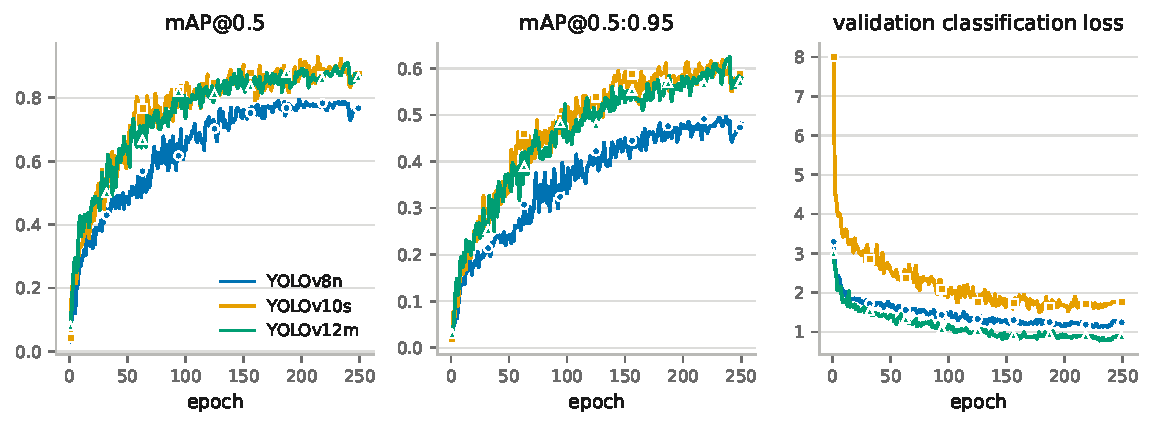
\includegraphics[width=\linewidth]{figures/training_curves.pdf}
\caption{Training trajectories. The epoch-to-epoch oscillation on a 23-image
validation split is comparable in size to the differences being compared.}
\label{fig:curves}
\end{figure}

\begin{figure}[t]
\centering
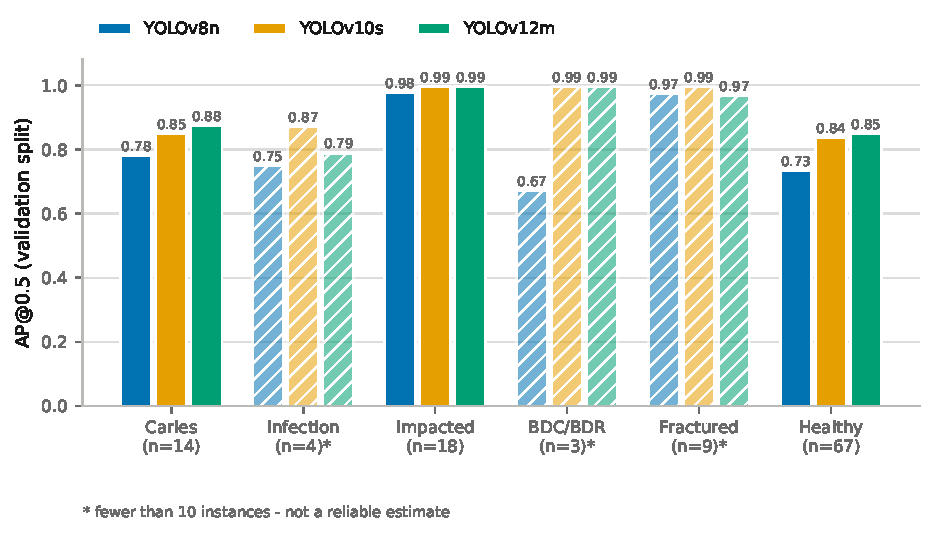
\includegraphics[width=\linewidth]{figures/per_class_ap50.pdf}
\caption{Per-class AP@0.5. Hatched bars mark classes with fewer than ten
validation instances. The tallest bars in the figure rest on the least data.}
\label{fig:perclass}
\end{figure}

\textbf{Error analysis.} The confusion structure of the YOLOv10s model is
unusually clean: inter-class confusion accounts for approximately 1\% of
predictions. Essentially every error is a missed detection or a background false
positive. Recall by class is \clsname{Impacted} 1.00, \clsname{BDC/BDR} 1.00,
\clsname{Fractured} 0.89, \clsname{Caries} 0.79, \clsname{Healthy} 0.64,
\clsname{Infection} 0.50; the complement of each is, in every case, ground truth
assigned to background rather than to a wrong class. Of the false positives
raised on background, 82\% are labelled \clsname{Healthy}, 9\%
\clsname{Caries} and 9\% \clsname{BDC/BDR}.

The interpretation is specific and actionable. The classification head is not the
bottleneck---given a proposal, the model names it correctly. The bottleneck is
proposal recall, concentrated on \clsname{Infection} (half of all periapical
radiolucencies are never proposed) and on \clsname{Healthy}, where the
overwhelming instance count paradoxically coincides with the worst
recall-to-background ratio, consistent with the detector treating unremarkable
tooth regions as background. This points at loss weighting, confidence
thresholding and input resolution rather than at the label taxonomy or the
classifier.

\section{Protocol and reproduction}

The audit above is a description of a problem; the repository accompanying this
report implements the fix in four command-line tools: \texttt{dataset.py}
(prepare, audit with leakage check, grouped rarity-aware fold construction),
\texttt{model.py} (multi-seed training, ablation, aggregation),
\texttt{evaluate.py} (per-class metrics with bootstrap intervals, head-to-head
comparison) and \texttt{evaluate\_new.py} (error decomposition, threshold
sweep, scored saliency). The
ablation grid is declared in YAML as deltas from the baseline recipe---eleven
augmentation and schedule variants plus four architectures---and every variant
is reported as mean $\pm$ standard deviation over seeds with Welch's $t$-test
and Cohen's $d$ against the baseline, so that ``moved the needle'' and ``within
noise'' are verdicts rather than adjectives. At $\sim$72\,min per YOLOv10s run
the full grid is roughly 60 GPU-hours; a 120-epoch first pass over three seeds
costs about a third of that and preserves the ranking of variants.

The hypotheses attached to each ablation are stated in advance in the config.
Two are worth flagging: mosaic augmentation composites four radiographs into
one, destroying the fixed global anatomy of a panoramic view, and may therefore
hurt on this modality despite being a reliable win on natural images; and HSV
jitter on a greyscale modality can only perturb value, so its hue and saturation
components are expected to be exactly inert.

\section{Limitations}

The single largest limitation is data. 231 radiographs from one source, with one
annotator and no inter-rater agreement statistics, cannot support a claim about
clinical performance in any population. The \clsname{Healthy} class is not a
condition but a background label, which makes the six-class mean a mixture of
two different tasks. No calibration analysis is reported: the confidence values
the interface displays have not been checked against empirical accuracy, and
should not be read as probabilities. The system is a research artefact and a
demonstration; it is not a diagnostic device and must not be used as one.

\section{Conclusion}

Decomposing a single mAP@0.5 of 0.92 into its six components showed that the
classes contributing most to it are the ones with the least evidence behind
them, that the ranking of the two leading architectures inverts depending on
which classes are counted, and that the model's residual error is almost
entirely missed detections rather than misclassification. The corrective is not
a better backbone but a protocol that the dataset can actually support: grouped
cross-validation, repeated seeds, per-class intervals, and explanations scored
rather than displayed.

\small
\bibliographystyle{plain}
\bibliography{refs}

\end{document}
